\chapter{Lecture}\label{part1:lec2}
\markboth{\thechapter. Lecture}{\thechapter. Lecture}

In\pageoriginale  the last lecture we proved the identity:
\begin{equation*}
  \prod\limits_{n=1}^\infty (1+ \mathfrak{z} x^k) =
  \sum\limits_{k=0}^\infty \mathfrak{z}^k A_k (x), \tag{1}\label{part1:lec2:eq1}
\end{equation*}
where
\begin{equation*}
A_k (x) = \frac{x^{k(k+1)/2}}{(1-x)(1-x^2)\cdots
    (1-x^k)}\tag{2}\label{part1:lec2:eq2}
\end{equation*}

We shall look upon the right side of (\ref{part1:lec2:eq1}) as a power series in $x$ and
\textit{not} as a power-series in $z$, as otherwise the infinite
product on the left side would have no sense in our formalism. Let us
interpret (\ref{part1:lec2:eq1}) arithmetically. If we want to decompose $m$ into $k$
summands, we have evidently to look for $\mathfrak{z}^k$ and then for
$x^m$, and the coefficient of $\mathfrak{z}^k x^m$ on the right side
of (\ref{part1:lec2:eq1}) gives us exactly what we want. We have
\begin{align*}
  \frac{1}{(1-x)(1-x^2)\cdots (1-x^k)} & = \sum_{n_1=0}^\infty
  x^{n_1} \sum_{n_2=0}^\infty x^{2n_2}\cdots
  \sum_{n_k=0}^\infty x^{kn_k}\hspace{2cm}\\
  & = \sum_{m=0}^\infty p_m^{(k)} x^m,\\
  \text{say, with} \hspace{2cm}  p_0^{(k)} & =1.
\end{align*}

Therefore $m$ occurs only in the form
$$
m=n_1 + 2n_2 + \cdots + kn_k, n_j \geq 0,
$$
and $p_m^{(k)}$ tells us how often $m$ can be represented by $k$
different summands (with possible repetitions). On the other hand the
coefficient of $x^m$ on the left-side of (\ref{part1:lec2:eq1}) gives us the number of
partitions of $m$ into summands not exceeding $k$. Hence,
\begin{thm}\label{part1:lec2:thm2} %%%% 2
  $m$\pageoriginale  can be represented as the sum of $k$ different parts as often as
  $m-\dfrac{k(k+1)}{2}$ can be expressed as the sum of parts not
  exceeding $k$ (repetition being allowed). 
\end{thm}

(In the first the number of parts is fixed, in the second, the size of
parts).

In a similar way, we can establish the identity
\begin{equation*}
  \frac{1}{\prod_{n=1}^\infty (1- \mathfrak{z}x^n)} =
  \sum_{k=0}^\infty \mathfrak{z}^k B_k (x), \tag{3}\label{part1:lec2:eq3}
\end{equation*}
with $B_0=1$, which again can be interpreted arithmetically as
follows. 

The left side is 
\begin{equation*}
\sum\limits_{n_1=0}^\infty (\mathfrak{z}x)^{n_1}
  \sum\limits_{n_2=0}^\infty  (\mathfrak{z} x^2)^{n_2}
  \sum\limits_{n_3=0}^\infty (\mathfrak{z}x^3)^{n_3} \cdots 
\end{equation*}
and
\begin{equation*}
  B_k(x) = \frac{x^k}{(1-x)(1-x^2) \cdots (1-x^k)}\tag{4}\label{part1:lec2:eq4}
\end{equation*}

The left-side of (\ref{part1:lec2:eq3}) gives $m$ with the representation
$$
m=n_1 + 2n_2 + 3n_3+ \cdots
$$
i.e., as a sum of parts with repetitions allowed. Exactly as above we
have:

\begin{thm}\label{part1:lec2:thm3}
  $m$ can be expressed as the sum of $k$ parts (repetitions allowed)
  as often as $m-k$ as the sum of parts not exceeding $k$.
\end{thm}

We shall now consider odd summands which will be of interest in
connexion with $\mathcal{V}$-function later. As earlier we can
establish the identity
\begin{equation*}
  \prod_{\mathcal{V}~\text{odd}} (1+ \mathfrak{z} x^{\mathcal{V}}) =
  \sum_{k=0}^\infty \mathfrak{z}^k C_k(x) \tag{5}\label{part1:lec2:eq5}
\end{equation*}
with\pageoriginale  the provide that $C_\circ (x)=1$. The trick is the same. One
studies temporarily a truncated affair
$\prod\limits_{\mathcal{V}=1}^V(1+ \mathfrak{z} x^{\mathcal{V}})$,
replaces $z$ by $\mathfrak{z}x^2$ and evaluates $C_k(x)$ as in Lecture
1. This would be perfectly legitimate. However one could proceed as
Euler did - this is not quite our story. Multiplying both sides by $1+
\mathfrak{z}x^2$, we have
$$
\sum\limits^\infty_{k=0} \mathfrak{z}^k C_k (x) = (1+\mathfrak{z}x^2)
\sum\limits^\infty_{k=0} \mathfrak{z}^k x^{2k} C_k (x).
$$

Now compare powers of $z$ on both sides - and this was what required
some extra thought. $C_k(x)$ begins with $x^{1+3+\cdots+(2k-1)}=
x^{k^2}$; in fact they begin with later and later powers of $x$ and so
can be added up. We have
\begin{align*}
  C_0 & =1,\\
  C_k(x) & = x^{2k} C_k (x) + x^{2k-1} C_{k-1} (x), k> 0,\hspace{2cm}\\
  \text{or} \hspace{2cm} C_k (x) & = \frac{x^{2k-1}}{1-x^{2k}} C_{k-1} (x)
\end{align*}
from this recurrence relation we obtain
\begin{align*}
  C_1(x) & = \frac{x}{1-x^2},\\
  C_2(x) & = \frac{x^3}{1-x^4} C_1 (x) = \frac{x^4}{(1-x^2)(1-x^4)},\\
  C_3 (x) & = \frac{x^5}{1-x^6}  C_2(x)= \frac{x^9}{(1-x^2)(1-x^4)(1-x^6)},\\
  & \dots \dots \dots \dots \dots\\
  & \dots \dots \dots \dots \dots\\
  C_k(x) & = \frac{x^{k^2}}{(1-x^2)(1-x^4)\cdots (1-x^{2k})},
\end{align*}
carrying on the same rigmarole.

Now note that all this can be retranslated into something.

Let\pageoriginale  us give the number theoretic interpretation. The coefficient of
$\mathfrak{z}^k x^m$ gives the number of times $m$ can be expressed as
the sum of $k$ different odd summands. On the other hand, the
coefficients in the expansion of $\frac{1}{(1-x^2)\cdots (1-x^{2k})}$
give the decomposition into even summands, with repetitions. Hence,

\begin{thm}\label{part1:lec2:thm4} %% 4
  $m$ is the sum of $k$ different odd parts as often as $m-k^2$ is the
  sum of even parts not exceeding $2k$, or what is the same thing, as
  $\frac{m-k^2}{2}$ is the sum of parts not exceeding $k$. (since $m$
  and $k$ are obviously of the same parity, it follows that
  $\frac{m-k^2}{2}$ is an integer).
\end{thm}

Finally we can prove that 
\begin{equation*}
  \frac{1}{\prod_{\mathcal{V} ~\text{odd}} (1-
    \mathfrak{z}x^\mathcal{V})} = \sum_{k=0}^\infty \mathfrak{z}^k
  D_k(x)\tag{6}\label{part1:lec2:eq6}
\end{equation*}

Replacing $\mathfrak{z}$ by $\mathfrak{z}x^2$, we obtain
$$
D_k (x) = \frac{x^k}{(1-x^2)\cdots (1-x^{2k})},
$$
leading to the 

\begin{thm}\label{part1:lec2:thm5} %%% 5
  $m$ is the sum of $k$ odd parts as often as $m-k$ is the sum of even
  parts not exceeding $2k$, or $\frac{m-k}{2}$ is the sum of even
  parts not exceeding $k$. ($\frac{m-k}{2}$ again is integral).
\end{thm}

\noindent \textbf{\large Some other methods}

Temporarily we give up power series and make use of graphs to study
partitions. A partition of $\mathcal{N}$ may be represented as an
array of dots, the number of dots in a row being equal to the
magnitude of a summand. Let us arrange the summands according to size.

For\pageoriginale  instance, let us consider a partition of 18 into 4 different parts

\begin{figure}[H]
\centering{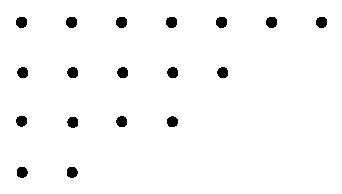
\includegraphics{vol2-figures/fig2.1.eps}}
\end{figure}

If we read the diagram by rows we get the partition $18=7+5+4+2$. On the
other hand reading by columns we have the petition $18=
4+4+3+3+2+1+1$. In general it is clear that if we represent a partition
of $n$ into $k$ parts graphically, then reading the graph vertically
yields a partition of $n$ with the largest part $k$, and
conversely. This method demonstrates a one-to-one correspondence
between partitions of $n$ with $k$ parts and partitions sees that the
number of partitions of $n$ with largest part $k$ is equal to the
number of partitions of $n-k$ into parts not exceeding $k$.

\begin{figure}[H]
\centering{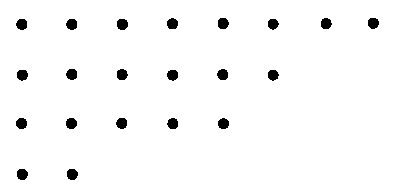
\includegraphics{vol2-figures/fig2.2.eps}}
\end{figure}

Draw a diagonal upward starting from the last but one dot in the
column on the extreme left. All the dots to the right of this diagonal
constitute a partition of 12 into 4 parts. For each partition of 18
into 4 different parts there corresponds thus a partition of $18-
\frac{4.3}{2} =12$ into parts. This process works in general for a\pageoriginale 
partition of $n$ with $k$ different parts. If we throw away the dots
on and to the left of the diagonal (which is drawn from the last but
one point from the bottom in order to ensure that the number of
different parts continues to be exactly $k$), we are left with a
partition of $n-(1+2+3+\cdots+ (k-1))=n- \frac{k(k-1)}{2}$. This
partition has exactly $k$ parts because each row is longer by at least
one dot than the row below it, so an entire row is never
discarded. Conversely, starting with a partition of
$n-\frac{k(k-1)}{2}$ into $k$ parts, we can build up a unique
partition of $n$ into $k$ different parts. Add 1 to the next to the
smallest part, 2 to the next longer, 3 to the next and so on. This
one-to-one correspondence proves that the number of partitions of $n$
into $k$ different parts equals the number of partitions of
$n-\frac{k(k-1)}{2}$ into $k$ parts.

We can prove graphically that the number of partitions of $n$ into $k$
odd summands is the same as the number of partitions of $n-k^2$ into
even summands not exceeding $k$. The last row of the 

\begin{figure}[H]
\centering{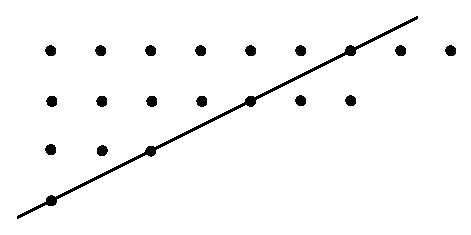
\includegraphics{vol2-figures/fig2.3.eps}}
\end{figure}
diagram contains at least one dot, the next higher at least three, the
one above at least five, and so on. Above and on the diagonal there
are $1+3+5+\cdots + (2k-1) =k^2$ dots. When these are removed, an even
number of dots is left in each row, altogether adding up to
$n-k^2$. This proves the result.

Theorem\pageoriginale  \ref{part1:lec1:thm1} can also be proved graphically, although the proof is not
quite as simple. The idea of the proof is exemplified by considering
the partitions of 35. We have
\begin{align*}
  35 & = 10+ 8+7+ 5+ 4+1\\
  & = 5 \times 2+1\times 8+7+5+1\times 4+1\\
  & = 5(2+1) +7\times 1+1(8+4+1)\\
  & 7+5 +5+5+\left(\mathop{\underbrace{1+\cdots +1}}_{13 ~\text{times}}\right)
\end{align*}

Thus to each unrestricted partition of 35 we can make correspond a
partition into add summands with possible repetitions. Conversely 
\begin{align*}
  7 \times 1 + 5 \times 3+ 1 \times 13 & = 7 \times 1 + 5(1+2) +1 (2^3 +
  2^2 + 2^0)\\
  & = 7+ 5 +10 +8 + 4+ 1.
\end{align*}

Now consider the following diagram
\begin{figure}[H]
\centering{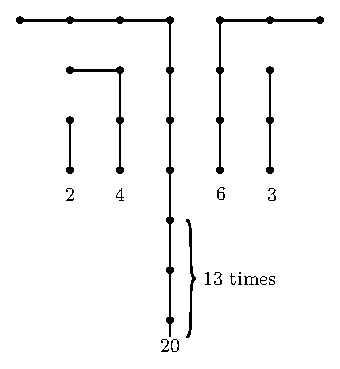
\includegraphics{vol2-figures/fig2.4.eps}}
\end{figure}

Each part is represented by a row of dots with the longest row at the
top, second longest next to the top, etc. The oddness of the parts
allows us to place the rows symmetrically about a central vertical
axis. Now\pageoriginale  connect the dots in the following way. Connect the dots on
this vertical axis with those on the left half of the top row. Then
connect the column to the right of this axis to the other half of the
top row. We continue in this way as indicated by the diagram drawing
right angles first on one side of the centre and then on the other. We
now interpret this diagram as a new partition of 35 each part being
represented by one of the lines indicated. In this way we obtain the
partition 20+6+4+3+2 of 35 into different parts. It can be proved that
this method works in general. That is, to prove that given a partition
of $n$ into odd parts, this method transforms it into a unique
partition of $n$ into distinct parts; conversely, given a partition
into distinct parts, the process can be reversed to find a unique
partition into odd parts. This establishes a one-to-one correspondence
between the two sorts of partitions. This proves our theorem.




